\documentclass{reportDoCS2025}

\usepackage{lmodern}
\usepackage{anyfontsize}

\addbibresource{biblio.bib}

%--------------------------------------
\university{ĐẠI HỌC QUỐC GIA TP. HỒ CHÍ MINH}
\school{TRƯỜNG ĐẠI HỌC KHOA HỌC TỰ NHIÊN}
\title{Ma Trận - Cơ sở của Tính Toán Khoa Học}
\subtitle{Báo Cáo Đồ Án Số 1 \\ Toán Ứng Dụng và Thống Kê - MTH00051}

\students{
    24120010 - Trần Văn Tấn Khôi \\
    24120028 - Cao Việt Cường \\
    24120035 - Lê Thành Đạt \\
    24120038 - Nguyễn Phú Đạt \\
    24120054 - Mai Phan Nhật Hoàng
}

\supervisors{
    Võ Nam Thục Đoan \\
    Lê Nhựt Nam
}

%--------------------------------------

\begin{document}

\cover
\numRoman

% \input{1.acknowledgements}

\contents
\listTables
\listImages

% \input{2.symbol_lists}

\pageNumber

\chapter{Phép Khử Gauss và Các Ứng Dụng}

\newpage

\section{<tên mục 1>}

\section{<tên mục 2>}

\chapter{Phân Rã Ma Trận Và Trực Quan Hóa Với Manim}

\newpage

\section{Phân rã giá trị suy biến (SVD)}

\subsection{Định nghĩa ma trận SVD}

Phân rã giá trị suy biến - Singular Value Decomposition là một công cụ mạnh mẽ trong đại số tuyến tính, nó cho phép phân tích một ma trận bất kỳ $A \in \mathbb{R}^{m \times n}$ thành ba ma trận đặc biệt:

{\large
\begin{equation}
    A = U \Sigma V^T
\end{equation}
}

Trong đó:

\begin{itemize}[topsep=0pt, itemsep=2.5pt, leftmargin=1.5cm]
    \item $U \in \mathbb{R}^{m \times m}$: Là ma trận trực giao ($U^TU=I_{m}$), các cột của nó là các vector suy biến trái.
    \item $\Sigma \in \mathbb{R}^{m \times n}$: Là ma trận đường chéo không vuông, chứa các giá trị suy biến $\sigma_{i}$ trên đường chéo chính.
    \item $V^T \in \mathbb{R}^{n \times n}$: Là ma trận trực giao ($V^TV = I_{n}$), các cột của nó là các vector suy biến phải.
\end{itemize}

\subsection{Tính chất của các giá trị suy biến}

\textbf{Thứ tự và dấu}: Các giá trị suy biến luôn không âm và thường được sắp xếp giảm dần.

\begin{equation}
    \sigma_1 \geq \sigma_2 \geq \dots \sigma_p \geq 0 \text{ với } p = min(m, n)
\end{equation}

\textbf{Hạng ma trận}: Số lượng các giá trị suy biến khác 0 tương ứng với hạng của ma trận $A$.

\textbf{Xấp xỉ hạng thấp}: SVD cung cấp xấp xỉ tốt nhất cho ma trận ở hạng $k$ thấp hơn qua công thức $A_k = \Sigma_{i = 1}^{k} \sigma_i u_i v_i^T$, ứng dụng trong nén ảnh và khử nhiều.

\subsection{Mối liên hệ với giá trị riêng (Eigenvalues)}

SVD là sự tổng quát hóa của phép chéo hóa, có mối quan hệ chặt chẽ với các giá trị riêng của ma trận đối xứng:

\begin{itemize}[topsep=0pt, itemsep=2.5pt, leftmargin=1.5cm]
    \item \textbf{Công thức liên hệ}: Các giá trị suy biến $\sigma_i$ của $A$ là căn bậc hai của các giá trị riêng $\lambda_i$ của ma trận $A^TA$:

    \begin{equation}
        \sigma_i = \sqrt{\lambda_i(A^TA)}
    \end{equation}

    \item \textbf{Cơ sở vector}: Các cột của $V$ là các vector riêng của $A^TA$, trong khi các cột của $U$ là các vector riêng của $AA^T$.
\end{itemize}

\section{Ý nghĩa của phân rã SVD}

\subsection{Cơ chế hoạt động}

SVD không chỉ đơn thuần là một công thức đại số, về mặt bản chất nó chính là một chuỗi các phép biến đổi hình học cơ bản. Bất kỳ ma trận $A$ nào cũng được đại diện cho một phép biến đổi tuyến tính từ không gian $\mathbb{R}^m$ sang không gian $\mathbb{R}^n$.

SVD cho phép phân tách phép biến đổi này thành ba bước độc lập:

\begin{itemize}[topsep=0pt, itemsep=2.5pt, leftmargin=1.5cm]
    \item Phép xoay đầu tiên ($V^T$): Ma trận trực giao $V^T$ thực hiện xoay hệ tọa độ trong không gian sao cho các trục tọa độ ban đầu trùng với các vector suy biến phải ($v_{i}$). Bước này không làm thay đổi độ dài của các vector.
    \item Phép co giãn ($\Sigma$): Ma trận đường chéo $\Sigma$ thực hiện co giãn theo không gian dọc theo các trục tọa độ mới. Các vector sẽ được co giãn hoặc rút ngắn theo các hệ số $\sigma_i$. Nếu $\sigma_i$, chiều không gian tương ứng bị triệt tiêu, điều đó giải thích vì sao mà SVD có thể xác định được hạng (rank) và không gian null (nullspace).
    \item Phép xoay thứ hai ($U$): Ma trận trực giao $U$ xoay hệ tọa độ một lần nữa trong không gian để đưa các vector về vị trí cuối cùng theo các vector suy biến trái.
\end{itemize}

\begin{figure}[h]
    \vspace{0.75cm}
    \centering
    \scalebox{1}{
        \begin{minipage}{\textwidth}
            \centering
            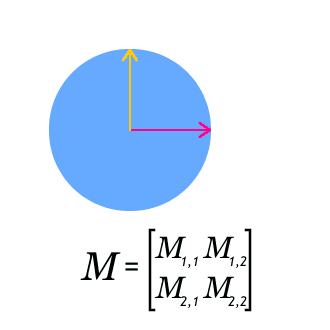
\includegraphics[width=0.25\textwidth]{images/chapter_02/svd-1.png}\hfill
            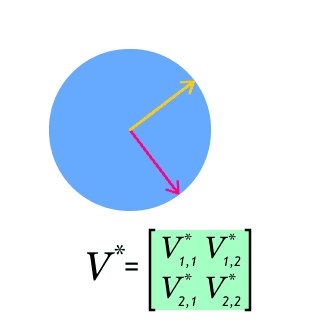
\includegraphics[width=0.25\textwidth]{images/chapter_02/svd-2.png}\hfill
            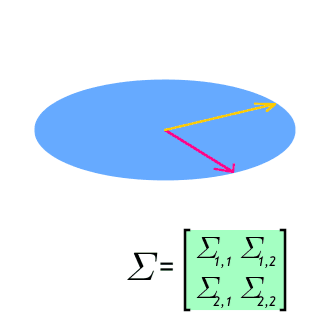
\includegraphics[width=0.25\textwidth]{images/chapter_02/svd-3.png}\hfill
            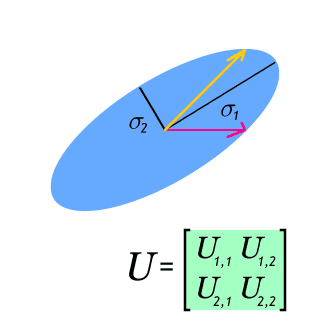
\includegraphics[width=0.25\textwidth]{images/chapter_02/svd-4.png}
        \end{minipage}
    }
    \caption{Các bước phân rã SVD}
    \label{fig:svd_decomp_steps}
\end{figure}

\newpage

\subsection{Vì sao cơ chế này quan trọng?}

Trong khi phép chéo hóa $A = PDP^{-1}$ chỉ hoạt động khi ta có thể tìm các trục mà tại đó ma trận chỉ thực hiện co giãn thì SVD chỉ ra rằng mọi ma trận (kể cả ma trận hình chữ nhật) đều có thể một cặp cơ sở trực chuẩn ($V$ và $U$) để biến hình cầu thành một hình ellipse.

Vì $U$ và $V$ là các ma trận trực giao, chúng không làm khuếch đại sai số tính toán làm cho thuật toán này trở nên ổn định nhất trong đại số tuyến tính. 

\section{Thuật toán giá trị riêng Jacobi}

\subsection{Định lý bất khả Abel}

Định lý phát biểu rằng \textbf{không tồn tại nghiệm đại số} - tức là nghiệm được biểu diễn bằng căn thức của phương trình đa thức tổng quát \textbf{bậc 5 hoặc lớn hơn} với các hệ số bất kỳ.

Trong quá trình tiến hành thuật toán SVD, chúng ta cần phải tìm các trị riêng của ma trận đối xứng $A^TA$. Việc tìm giá trị riêng tương đương với việc tìm nghiệm của đa thức đặc trưng $P(\lambda) = det(A - \lambda I) = 0$ nên đối với các ma trận có kích thước $\geq 5$, chúng ta không thể sử dụng các phương pháp đại số thông thường để giải quyết bài toán trên.

Dựa trên giới hạn của định lý Abel, ta phải sử dụng các phương pháp lặp số trị để giải quyết bài toán trên. Thuật toán Jacobi là lựa chọn tối ưu cho ma trận đối xứng vì:

\begin{itemize}[topsep=0pt, itemsep=2.5pt, leftmargin=1.5cm]
    \item Nó triệt tiêu các phần tử ngoài đường chéo bằng các phép xoay cho đến khi ma trận dần hội tụ về dạng đường chéo.
    \item Đảm bảo tính số học cao, phù hợp với yêu cầu ổn định số học của đồ án.
\end{itemize}

\newpage

\subsection{Chi tiết thuật toán}

\subsubsection{Phép xoay Jacobi}

Tại mỗi bước lặp, thuật toán chọn một phần tử ngoài đường chéo $s_{ij}$ (thường là phần tử có giá trị tuyệt đối lớn nhất) và triệt tiêu nó về 0 bằng một phép xoay trực giao, gọi là \textbf{ma trận xoay Jacobi} $G(i, j, \theta)$.

Ma trận $G$ giống với ma trận đơn vị nhưng có phần tử thay đổi tại bốn vị trí: $g_{ii}, g_{jj}, g_{ij} \text{ và } g_{ji}$. Khi đó, ma trận được cập nhật theo công thức: $S' = G^T S G$.

\begin{equation}
    \scalebox{0.9}{
    $
    G(i, j, \theta) = 
    \begin{bmatrix}
    1 &        &          & \text{\small Cột $i$} &        & \text{\small Cột $j$} &   \\
    & \ddots &          & \downarrow          &        & \downarrow                 &   \\
    &        & 1        &                     &        &                            &   \\
    &        &          & \cos\theta          & \dots  & -\sin\theta                & \rightarrow \text{\small Dòng $i$} \\
    &        &          & \vdots              & 1      & \vdots                     &   \\
    &        &          & \sin\theta          & \dots  & \cos\theta                 & \rightarrow \text{\small Dòng $j$} \\
    &        &          &                     &        & 1                          &   \\
    &        &          &                     &        &        & \ddots             &   \\
    &        &          &                     &        &        &                    & 1
    \end{bmatrix}
    $
    }
\end{equation}

Vì $G$ là ma trận trực giao nên phép biến đổi trên giữ nguyên đa thức đặc trưng của ma trận. Tức là $S$ và $S'$ có cùng tập hợp các trị riêng. Do đó mà ta có thể lặp lại quá trình mà vẫn giữ được các trị riêng ban đầu của $A^TA$.

Không những thế, ma trận trực giao $G$ có đặc tính bảo toàn bình phương tất cả các phần tử. Khi phép quay làm một phần tử ngoài đường chéo triệt tiêu về 0, giá trị đó không biến mất mà được "đẩy" vào các phần tử trên đường chéo chính.

\subsubsection{Tính toán góc xoay $\theta$}

Để phần tử $s_{ij}'$ trở về bằng $0$ sau phép biến đổi, góc $\theta$ được xác định dựa trên các phần tử hiện tại của ma trận $S$:

\begin{itemize}[topsep=0pt, itemsep=2.5pt, leftmargin=1.5cm]
    \item Nếu $s_{ii} = s_{jj}$ thì $\theta = \pi/4$.
    \item Nếu $s{ii} \neq s_{jj}$, ta tính $\theta$ thông qua giá trị $\tau = \frac{s_{jj} - s_{ii}}{2s_{ij}}$, sau đó tìm $t = tan(\theta)$ là nghiệm của phương trình $t^2 + 2rt - 1 = 0$.
\end{itemize}

\newpage

\subsubsection{Các bước thực hiện thuật toán}

\begin{algorithm}[H]
\caption{\textproc{Thuật toán trị riêng Jacobi}}
\begin{algorithmic}[1]
\Procedure{jacobi\_eigenvalues(A, $\epsilon$, max\_iter)}{}
    \State $S \gets A^TA$, $V \gets I_n$
    
    \State $is\_converge \gets False$

    \While{$is\_converge$}
        \State $max\_val \gets max(s_{ij}) \quad (i \neq j)$
        \If{$|s_{ij}| < \epsilon$ (với $\epsilon$ là ngưỡng sai số cực nhỏ)}
            \State $is\_converge \gets True$
            \State \textbf{break}
        \EndIf
        \State $cos(\theta), sin(\theta) \text{ được tính từ } s_{ii}, s_{jj}, s_{ij}$
        \State $S \gets G^T S G$ (ma trận $S$ dần trở thành ma trận đường chéo $\Sigma^2$)
        \State $V \gets V G$ (các cột của $V$ dần trở thành vector suy biến phải)
    \EndWhile
    \State $eigenvalues \gets \text{Các phần tử trên đường chéo chính của } S$
    \State \Return $eigenvalues, V$
\EndProcedure
\end{algorithmic}
\end{algorithm}

\newpage

\section{Chéo hóa ma trận}

\subsection{Cơ sở lý thuyết}

Một ma trận vuông $A \in \mathbb{R}^{n \times n}$ được gọi là chéo hóa được nếu tồn tại một ma trận khả nghịch $P$ và một ma trận đường chéo $D$ sao cho:

{\large
\begin{equation}
    A = PDP^{-1}
\end{equation}
}

Trong đó:

\begin{itemize}[topsep=0pt, itemsep=2.5pt, leftmargin=1.5cm]
    \item D là ma trận đường chéo $diag(\lambda_1, \lambda_2, \dots, \lambda_i)$ với $\lambda_i$ là các giá trị riêng của $A$.
    \item P là ma trận các vector riêng, trong đó mỗi cột của $P$ là một vector riêng ứng với giá trị riêng $\lambda_i$.
\end{itemize}

Quá trình chéo hóa phụ thuộc hoàn toàn vào việc tìm kiếm các đặc trưng phổ của ma trận:

\begin{itemize}[topsep=0pt, itemsep=2.5pt, leftmargin=1.5cm]
    \item \textbf{Trị riêng} $\lambda$: Trị riêng được xác định từ phương trình đặc trưng $det(A - \lambda I) = 0$. Đây là giá trị vô hướng thể hiện mức độ co giãn của ma trận theo một hướng nhất định.
    \item \textbf{Vector riêng} $x$: Vector riêng tương ứng là nghiệm của hệ $(A - \lambda I) = 0$. Nó đại diện cho hướng mà tại đó phép biến đổi tuyến tính chỉ đóng vai trò như phép nhân vô hướng.
    \item \textbf{Điều kiện chéo hóa}: Ma trận $A \in \mathbb{R}^{n \times n}$ chéo hóa được khi và chỉ khi tồn tại đủ $n$ vector riêng độc lập tuyến tính để cấu thành các cột của ma trận khả nghịch $P$.
\end{itemize}

\subsection{Trường hợp đặc biệt: Ma trận đối xứng thực}

\subsubsection{Định lý phổ (Spectral Theorem)}

Đối với ma trận vuông bất kỳ, việc chéo hóa được hay không phụ thuộc vào số lượng vector riêng độc lập tuyến tính. Tuy nhiên đối với ma trận đối xứng thực $A$, định lý phổ khẳng định:

\begin{itemize}[topsep=0pt, itemsep=2.5pt, leftmargin=1.5cm]
    \item $A$ \textbf{luôn} chéo hóa được.
    \item Tất cả các trị riêng của $A$ đều là \textbf{số thực}.
    \item Các vector riêng ứng với các giá trị riêng khác nhau của $A$ luôn \textbf{trực giao} với nhau.
\end{itemize}

\subsubsection{Chéo hóa trực giao}

Vì các vector riêng của ma trận đối xứng thực có thể chọn để tạo thành một bộ cơ sở trực chuẩn, công thức chéo hóa trở thành:

{\large
\begin{equation}
    A = QDQ^{-1}
\end{equation}
}

Trong đó:

\begin{itemize}[topsep=0pt, itemsep=2.5pt, leftmargin=1.5cm]
    \item $Q$ là ma trận trực giao thỏa mãn $Q^{-1} = Q^T$. Điều này giúp việc tính toán ma trận nghịch đảo trở nên đơn giản bằng một phép chuyển vị thay vì tốn chi phí $O(n^3)$ thông thường với ma trận $P$.
    \item $D$ là ma trận đường chéo chứa các trị riêng của $A$. 
\end{itemize}

\subsubsection{Vai trò và ý nghĩa trong tính toán}

\begin{itemize}[topsep=0pt, itemsep=2.5pt, leftmargin=1.5cm]
    \item \textbf{Sự ổn định}: Các phép biển đổi trực giao không làm khuếch đại sai số làm tròn, đảm bảo độ chính xác cực kỳ cao ($< 10^{-10}$) khi xử lý trong thực tế.
    \item \textbf{Mối liên hệ với SVD}: Đây là sự kết nối trực tiếp đến phân rã SVD. Trong SVD, chúng ta phải thực hiện chéo hóa ma trận đối xứng $A^TA$ để tìm các giá trị suy biến và vector suy biến phải. 
    \item \textbf{Tối ưu hiệu năng}: Đối với ma trận đối xứng xác định dương, chi phí tính toán có thể giảm xuống bằng một nửa so với các phương pháp thông thường.
\end{itemize}

\section{Phương pháp tìm trị riêng và vector riêng}

    

\newpage

\section{Trực quan hóa với Manim}
\chapter{Giải Hệ Phương Trình Và Phân Tích Hiệu Năng}

\newpage

\section{Cơ sở lý thuyết}
Phân tích hiệu năng của các thuật toán giải hệ $Ax = b$ được xây dựng trên sự tương tác giữa đặc tính cấu trúc của ma trận và triết lý tính toán của thuật toán.

\begin{itemize}[topsep=0pt, itemsep=2.5pt, leftmargin=1.5cm]
    \item Ma trận Đối xứng Xác định Dương (SPD): Sở hữu phổ trị riêng thực dương ($\lambda_i > 0$). Các hệ SPD thực tế thường được khống chế tốt (well-conditioned), đóng vai trò như một "bộ giảm xóc số học", phong tỏa sự khuếch đại nhiễu và đảm bảo sự hội tụ cho phương pháp lặp.
    \item Ma trận Hilbert: Nguyên mẫu kinh điển của sự suy biến cực đoan (ill-conditioned). Dù mang cấu trúc SPD, các trị riêng của nó phân rã về $0$ theo hàm mũ, khiến định thức tiệm cận $0$.
    \item Số điều kiện ($\kappa(A)$): Thước đo độ nhạy hệ thống (với SPD, $\kappa = \lambda_{max}/\lambda_{min}$). Theo định lý nhiễu loạn, sai số nghiệm tỷ lệ thuận với $\kappa$. Trên hệ Hilbert, $\kappa$ bùng nổ vượt quá giới hạn biểu diễn của số thực 64-bit, trở thành thứ phá hủy mọi nỗ lực tính toán.
\end{itemize}

Các bộ giải được chia thành hai trường phái, đối mặt với sự suy biến theo những cách khác biệt:

\begin{itemize}[topsep=0pt, itemsep=2.5pt, leftmargin=1.5cm]
    \item Nhóm Phương pháp Trực tiếp (Direct Methods)
    Đặc trưng bởi tính tất định, giải bài toán trong số bước $\mathcal{O}(N^3)$ hữu hạn, nhưng phải chịu "thuế tích lũy sai số cơ học":
    \begin{itemize}[label=\ding{111}, leftmargin=1.5cm]
        \item Khử Gauss ($A=LU$): Tối ưu hóa tốc độ phần cứng cực tốt nhưng sử dụng các biến đổi không trực giao. Rất dễ bị phá hủy bởi hiện tượng sụp đổ phần tử trục (pivot collapse) và khuếch đại nhiễu trên ma trận xấu.
        \item Phân rã SVD ($A=U\Sigma V^T$): Tiêu chuẩn vàng về độ ổn định ngược. Các phép biến đổi trực giao đẳng cự ($\kappa=1$) giúp SVD không bao giờ tự sinh/khuếch đại rác số học. Điểm yếu là chi phí tính toán siêu việt khổng lồ và dễ mất toàn bộ tính ổn định nếu lập trình ngây thơ qua bước nhân hiệp phương sai $A^T A$.
    \end{itemize}
    \item Phương pháp Lặp (Iterative Methods): Gauss-Seidel: Khả năng hội tụ bị quyết định tuyệt đối bởi bán kính phổ của ma trận lặp ($\rho < 1$). Trên hệ SPD lý tưởng, thuật toán tạo ra cơ chế nén sai số chủ động. Tuy nhiên, trên hệ suy biến như Hilbert, do $\rho \to 1$, động năng tiệm cận bị triệt tiêu hoàn toàn, ép hệ thống rơi vào trạng thái đình trệ giải tích (stagnation) vĩnh viễn.
\end{itemize}

\section{Phân tích hiệu năng}
Qua quá trình đối chiếu thực nghiệm trên hai hệ không gian đối lập (SPD khống chế tốt và Hilbert khống chế cực kém), hiệu năng của ba bộ giải tuyến tính bộc lộ rõ bản chất đánh đổi tàn khốc của Giải tích số:

\begin{figure}[h!]
    \centering
    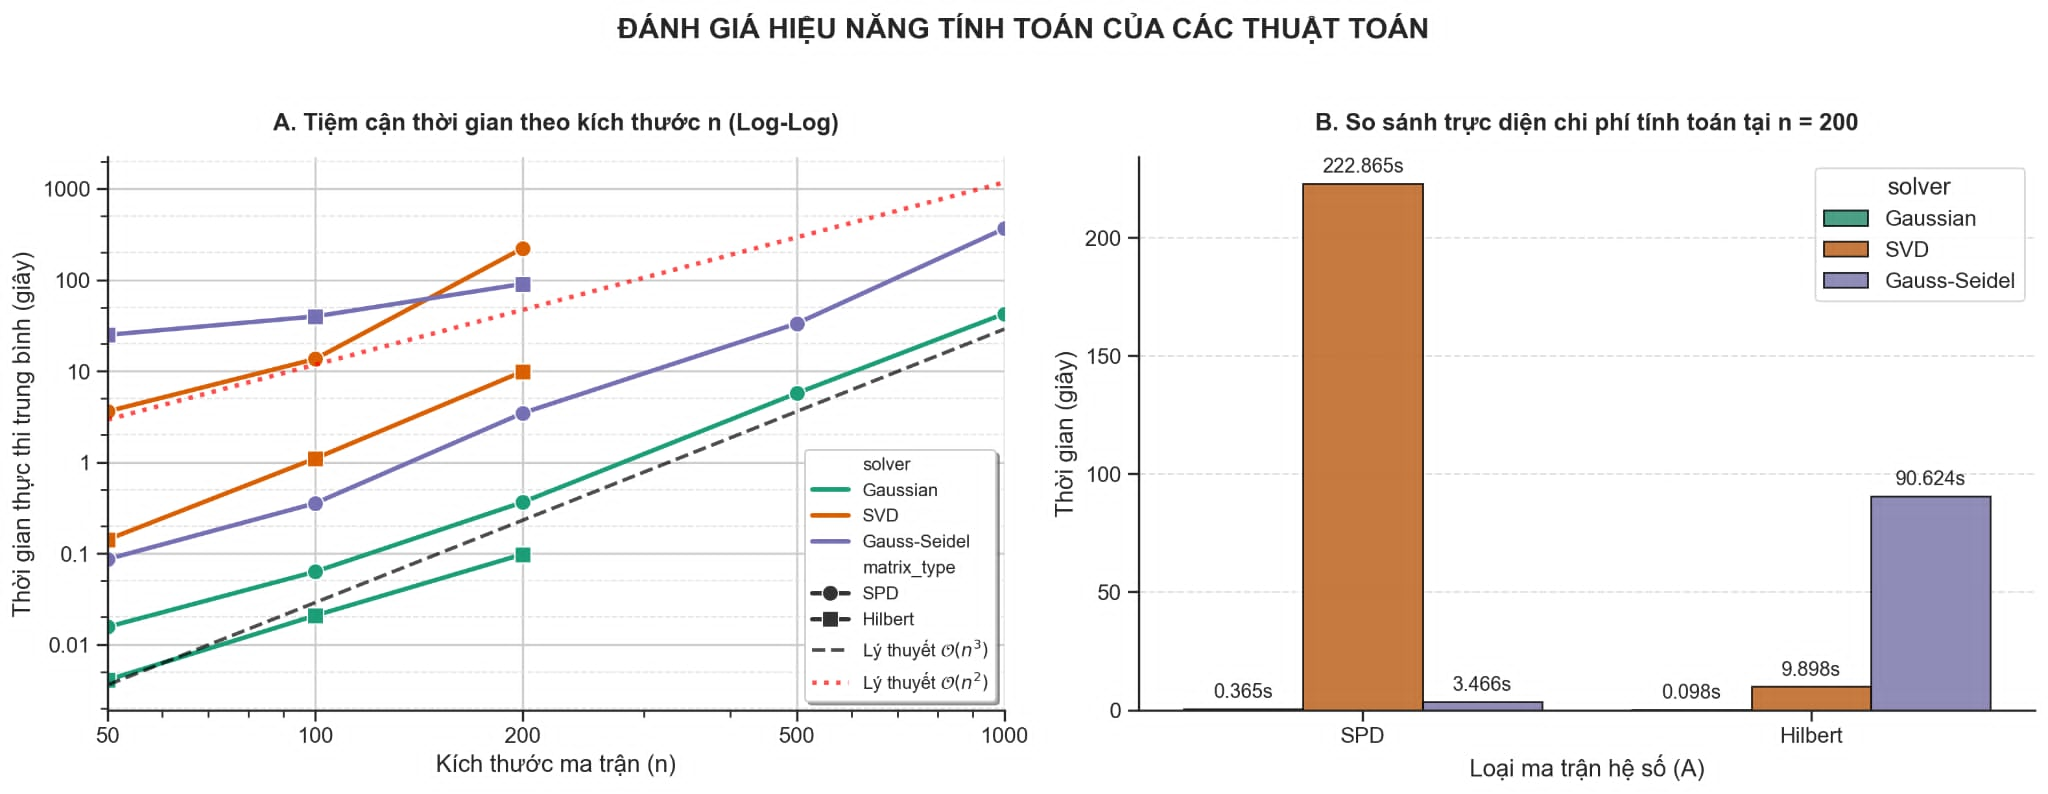
\includegraphics[width=1.0\textwidth]{images/chapter_03/time-execute.png}
    \caption{Thời gian thực thi}
    \label{fig:niuq}
\end{figure}

\begin{itemize}[topsep=0pt, itemsep=2.5pt, leftmargin=1.5cm]
    \item Khử Gauss (Đỉnh cao Tốc độ & Vực thẳm Suy biến): Đại diện cho sự tối ưu hóa vi kiến trúc cực đại với các lệnh FMA (nhân-cộng), cho thời gian thực thi nhanh nhất. Tuy nhiên, phép biến đổi không trực giao khiến nó trở thành nạn nhân của sự bào mòn sai số cơ học $\mathcal{O}(N^3)$. Trên không gian suy biến (Hilbert), sự sụp đổ của phần tử trục tạo ra Thảm họa Bùng nổ Sai số, phá hủy hoàn toàn cả phần dư lẫn vector nghiệm.
    \item SVD (Hàng rào Hình học & Lỗ hổng Triển khai): Được thiết kế như một tấm khiên tuyệt đối chống lại nhiễu nội sinh nhờ các phép quay trực giao đẳng cự. Tuy nhiên, phương pháp này chịu hình phạt khổng lồ về thời gian chạy do độ phức tạp của hàm siêu việt. Nghiêm trọng hơn, thực nghiệm chứng minh SVD rất mong manh trước lỗi cài đặt: Việc khởi tạo gián tiếp qua hiệp phương sai $A^T A$ đã châm ngòi cho hiện tượng Tràn số dưới (Underflow), dẫn đến Thất bại Tĩnh lặng (Hội tụ giả) trên hệ Hilbert và đánh mất hoàn toàn lợi thế chính xác lý tưởng.
    \item Gauss-Seidel (Kiểm soát Chủ động & Đình trệ Phổ): Đại diện cho triết lý hậu kiểm mục tiêu. Trên hệ ổn định (SPD), việc sử dụng chuẩn $L_2$ giúp thuật toán tạo ra Hiệu ứng Nén Sai số, ép buộc các biến số phải chính xác hơn khi không gian mở rộng (đánh đổi bằng chi phí lặp). Dẫu vậy, khi đối mặt với hệ suy biến ($\rho \to 1$), động năng hội tụ bị triệt tiêu, ép hệ thống vào trạng thái Đình trệ Giải tích. Sự đình trệ này, kết hợp với hiệu ứng bình phương nhiễu trắng của chuẩn $L_2$, vô tình đánh lừa các tiêu chuẩn dừng, khiến thuật toán nghiệm thu các "nghiệm rác" mà không hề hay biết.
\end{itemize}

Thực nghiệm khẳng định một tiên đề tối thượng trong Khoa học máy tính: Không tồn tại một thuật toán hoàn hảo cho mọi không gian dữ liệu. Trong khi Phương pháp Trực tiếp bị giới hạn bởi sự tích lũy nhiễu cơ học $\mathcal{O}(N^3)$, thì Phương pháp Lặp bị trói buộc bởi động năng của Bán kính phổ. Hơn thế nữa, dù thuật toán có thiết lập hàng rào phòng thủ vững chắc đến đâu (như SVD), giải tích số vĩnh viễn không thể vượt qua ranh giới vật lý áp đặt bởi Số điều kiện $\kappa(A)$ của ma trận. Lựa chọn bộ giải là nghệ thuật đánh đổi giữa Tốc độ Vi kiến trúc, Độ ổn định Hình học và Sự thấu hiểu sâu sắc về Độ nhạy Hệ thống.

\section{Phân tích độ ổn định}

\subsection{Hệ ma trận SPD (well-conditioned)}

Nhằm làm rõ bản chất thực sự của các bộ giải tuyến tính, phần dưới đây sẽ đi sâu phân tích biểu đồ quỹ đạo sai số trên không gian ma trận khống chế tốt (SPD). Việc đặt các thuật toán vào một môi trường dữ liệu hoàn hảo sẽ bóc trần một nghịch lý thú vị của Giải tích số: phương pháp được thiết kế với rào chắn an toàn cao nhất lại không phải là phương pháp chạm đến đáy sai số của máy tính

\begin{figure}[h!]
    \centering
    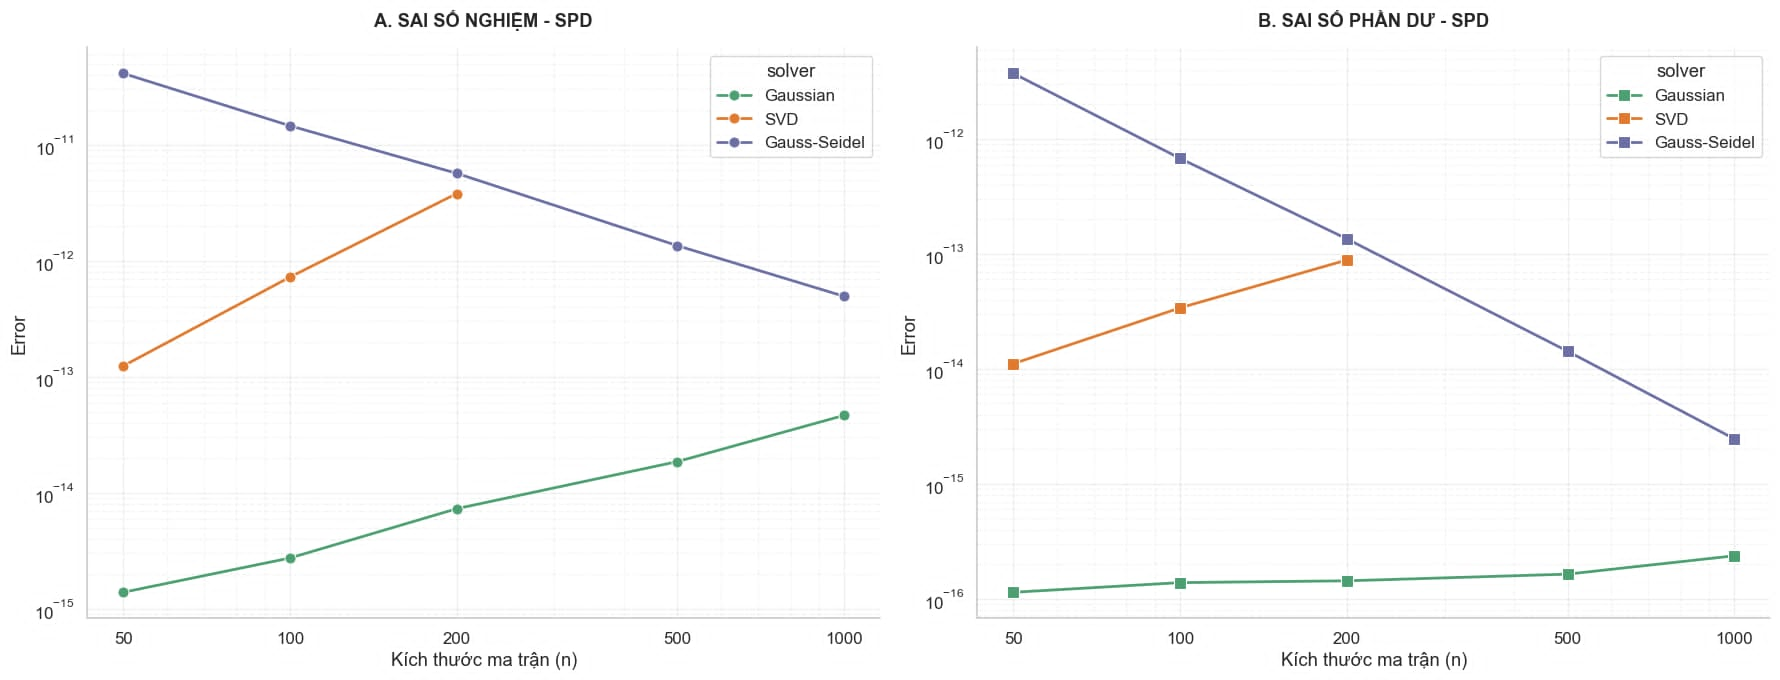
\includegraphics[width=1.0\textwidth]{images/chapter_03/spd.png} % <- path tới cái image / xóa dấu .. trong path đi
    \caption{Sai số trên hệ SPD} % <- caption là gì m / dòng chữ dưới tấm hình
    \label{fig:niuq} % vậy label là gì / này t ko bt, xóa cũng đc
\end{figure}

\begin{itemize}[topsep=0pt, itemsep=2.5pt, leftmargin=1.5cm]
    \item Khử Gauss (Tối ưu Vi kiến trúc & Chạm đáy Phần cứng): Được bảo chứng độ an toàn tuyệt đối bởi cấu trúc SPD (không xảy ra sụp đổ phần tử trục), thuật toán tận dụng tối đa tốc độ của tập lệnh nhân-cộng cơ sở (FMA) để vắt kiệt năng lực tính toán của Float64, đưa vector nghiệm cắm thẳng xuống và neo chặt tại giới hạn sai số tận cùng của máy tính (Machine Epsilon $\approx 10^{-16}$).
    \item SVD (Thuế Lượng giác & Suy hao Biến đổi): Mặc dù được bảo vệ bởi phép quay trực giao lý tưởng, thuật toán vẫn phải chịu mức sai số cao hơn Khử Gauss do gánh chịu "thuế tích lũy cơ học" sinh ra từ $\mathcal{O}(N^3)$ phép tính hàm siêu việt (lượng giác), cộng hưởng với lượng thông tin bị suy hao ngay từ bước nhân ma trận hiệp phương sai $A^T A$ sơ khởi.
    \item Gauss-Seidel (Kiểm soát Chủ động & Giới hạn Tiêu chuẩn): Thể hiện triết lý tối ưu thực dụng khi lơ lửng ở mức sai số cao nhất trên đồ thị không phải do bất ổn, mà do cơ chế hậu kiểm $L_2$ đã chủ động dừng thuật toán ngay khi vừa chạm ngưỡng dung sai (tolerance) do con người áp đặt, thành công trong việc tiết kiệm tài nguyên lặp và từ chối việc chạy đua độ chính xác dư thừa.
\end{itemize}

Trên một không gian dữ liệu lý tưởng như SPD, các giới hạn toán học lùi lại phía sau, nhường chỗ cho ranh giới của phần cứng và triết lý lập trình. Khử Gauss vươn tới giới hạn tuyệt đối của máy móc, SVD chịu thuế nhiễu loạn của khối lượng tính toán, trong khi Gauss-Seidel dừng lại ở giới hạn của nhu cầu thực tiễn.

\subsection{Hệ ma trận Hillbert (ill-conditioned)}

\subsubsection{Phương pháp Trực tiếp (Direct Methods)}

Nhóm phương pháp trực tiếp, đại diện tiêu biểu bởi thuật toán Khử Gauss và Phân rã giá trị suy biến (SVD), được xây dựng trên triết lý giải tích tất định: cam kết tìm ra nghiệm chính xác thông qua một chuỗi hữu hạn các phép phân rã cấu trúc ma trận. Phần dưới đây sẽ đi sâu phân tích cơ chế hoạt động của nhóm thuật toán này, làm rõ sự đánh đổi khốc liệt giữa lợi thế tối ưu hóa vi kiến trúc phần cứng và rủi ro tàn khốc của việc tích lũy sai số cơ học $\mathcal{O}(N^3)$ khi không gian tính toán mở rộng

\begin{figure}[h!]
    \centering
    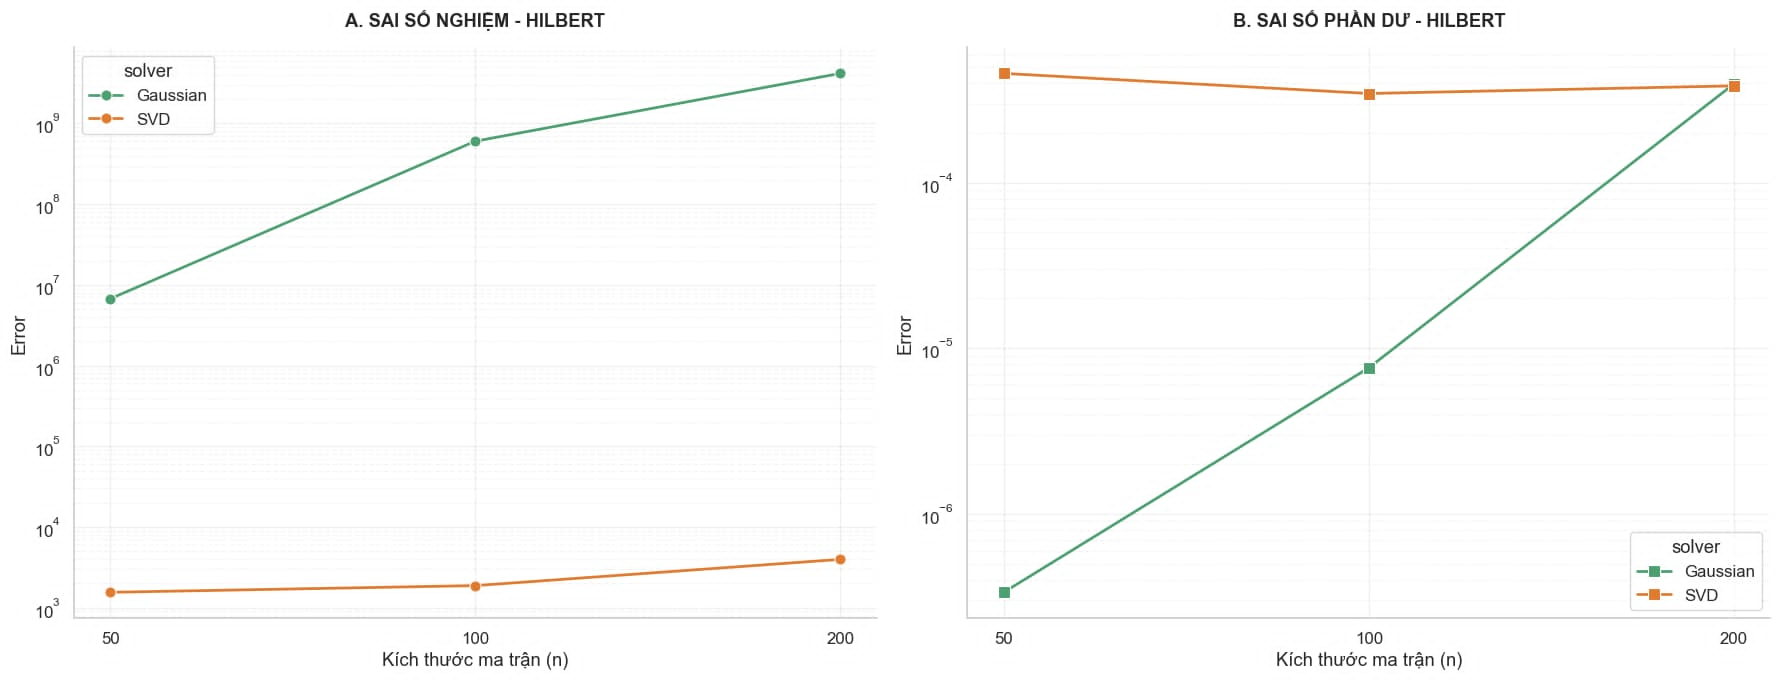
\includegraphics[width=1.0\textwidth]{images/chapter_03/hillbert.png} % <- path tới cái image / xóa dấu .. trong path đi
    \caption{Sai số trên hệ Hillbert} % <- caption là gì m / dòng chữ dưới tấm hình
    \label{fig:niuq} % vậy label là gì / này t ko bt, xóa cũng đc
\end{figure}

\begin{itemize}[topsep=0pt, itemsep=2.5pt, leftmargin=1.5cm]
    \item Khử Gauss (Đỉnh cao Vi kiến trúc & Vực thẳm Số học): Trên hệ SPD, Khử Gauss thống trị tuyệt đối về tốc độ nhờ tối ưu hóa lệnh FMA, vắt kiệt năng lực phần cứng để chạm đáy sai số Machine Epsilon ($10^{-16}$). Tuy nhiên, phép biến đổi không trực giao khiến nó sụp đổ tàn khốc trên hệ Hilbert: sự sụp đổ của phần tử trục tạo ra lượng rác số học khổng lồ, bùng nổ phi mã qua hệ số khuếch đại $\kappa$, phá hủy hoàn toàn cả vector nghiệm lẫn phần dư.
    \item SVD (Ảo ảnh Trực giao & Lỗ hổng Triển khai): SVD dùng phép quay trực giao ($\kappa=1$) để khóa chặt rác nội sinh, duy trì sự ổn định lý thuyết. Tuy nhiên, nó phải trả "thuế độ phức tạp" khổng lồ cho các phép toán lượng giác. Trầm trọng hơn, việc triển khai SVD gián tiếp qua $A^T A$ đã tự triệt tiêu thông tin ma trận, gây tràn số dưới (underflow) trên hệ Hilbert, dẫn đến "Thất bại tĩnh lặng" (hội tụ giả) thay vì một sự bảo vệ hình học như lý thuyết hứa hẹn.
\end{itemize}

\subsubsection{Phương pháp Lặp (Iterative Methods)}

Gauss-Seidel (Cơ chế Nén Chủ động & Bẫy Đình trệ Giải tích):

Trên hệ SPD, tiêu chuẩn chuẩn $L_2$ tạo ra "Hiệu ứng nén sai số", ép buộc hệ thống tự động thắt chặt độ chính xác của từng biến số cho đến khi lọt qua ngưỡng dung sai (tolerance) do con người áp đặt. Tuy nhiên, phương pháp lặp hoàn toàn bất lực trước sự biến dạng không gian. Trên hệ Hilbert, khi bán kính phổ tiệm cận 1 ($\rho \to 1$), động năng hội tụ bị triệt tiêu. Hệ thống rơi vào "Đình trệ giải tích", kết hợp với hiệu ứng underflow của việc bình phương chuẩn $L_2$, vô tình đánh lừa thuật toán nghiệm thu một vector rác trong sự cạn kiệt của tài nguyên thời gian (max_iter).

\section{Kết luận}
Thông qua việc đối chiếu hành vi của các bộ giải trên hai hệ không gian đối lập, thực nghiệm đã chứng minh một chân lý cốt lõi của Giải tích số: Độ ổn định của một nghiệm cuối cùng không được quyết định bởi sự ưu việt của thuật toán, mà bị chi phối tuyệt đối bởi bản chất của không gian ma trận. Sự phân hóa này được thể hiện qua hai thái cực:

\begin{itemize}[topsep=0pt, itemsep=2.5pt, leftmargin=1.5cm]
    \item Ma trận SPD (Vùng an toàn của Vi kiến trúc): Với đặc tính đối xứng và được khống chế tốt (số điều kiện $\kappa$ nhỏ), hệ SPD hoạt động như một "bộ giảm xóc số học" hoàn hảo. Nó phong tỏa sự khuếch đại sai số, cho phép các thuật toán bộc lộ tối đa năng lực lý thuyết của mình. Tại đây, Khử Gauss vươn tới giới hạn tột cùng của phần cứng (Machine Epsilon), SVD duy trì sự ổn định trực giao, và Gauss-Seidel hội tụ an toàn về đúng ngưỡng dung sai mục tiêu. Trên không gian này, rào cản duy nhất là giới hạn vật lý của máy tính và nhu cầu của con người.
    \item Ma trận Hilbert (Bản án của Sự suy biến):Trái ngược hoàn toàn, hệ Hilbert đại diện cho sự bóp méo thông tin cực đoan. Số điều kiện khổng lồ ($\kappa \approx 10^{19}$) trở thành một lăng kính khuếch đại tàn nhẫn, biến những nhiễu loạn cơ học vi mô thành thảm họa vĩ mô. Tại đây, mọi lưới bảo vệ của thuật toán đều bị xé toạc: Khử Gauss chết vì bùng nổ rác nội sinh, SVD chết vì tràn số dưới, và Gauss-Seidel chết vì đình trệ động năng. Không một kỹ thuật tối ưu mã nguồn nào có thể cứu vãn được hệ thống.
\end{itemize}

\chapter{Kết Luận}

\newpage

\section{Tóm tắt kết quả đạt được}

Trong khuôn khổ đồ án này, nhóm đã nghiên cứu và triển khai các phương pháp cốt lõi trong đại số tuyến tính, tập trung vào hai hướng chính: \textbf{giải hệ phương trình tuyến tính bằng phép khử Gauss} và \textbf{phân rã ma trận sử dụng phương pháp phân rã giá trị suy biến SVD}.

Ở phần 1, nhóm đã xây dựng thành công các thuật toán dựa trên phép khử Gauss, bao gồm giải hệ phương trình, tính định thức, tìm ma trận nghịch đảo, xác định hạng và không gian con. Việc áp dụng kỹ thuật \textbf{partial pivoting} giúp cải thiện độ ổn định số học. Kết quả thực nghiệm cho thấy các thuật toán được cài đặt có sai số rất nhỏ (xấp xỉ $10^{-6}$) khi so sánh với thư viện Numpy.

Ở phần 2, nhóm đã tiếp cận một trong những thuật toán phân rã ma trận phổ biến nhất - SVD, đồng thời nhóm cũng đã tìm hiểu thêm một số thuật toán tìm trị riêng như Jacobi và QR. Không chỉ dừng lại ở việc trình bày lý thuyết, nhóm đã tìm hiểu sâu về bản chất hình học của các phép biến đổi tuyến tính. Việc sử dụng Manim để trực quan hóa đã giúp truyền tải các khái niệm trừu tượng thành các hình ảnh sinh động, góp phần nâng cao khả năng tiếp cận và hiểu rõ bản chất phép phân rã.

Ở phần 3, nhóm đã tiến hành phân tích hiệu năng và độ ổn định của các thuật toán đã xây dựng thông qua thực nghiệm. Kết quả cho thấy thời gian thực thi của các phương pháp phù hợp với độ phức tạp lý thuyết, đồng thời các thuật toán trên hoạt động hiệu quả hơn trên các ma trận có điều kiện tốt (SPD) với sai số rất nhỏ. Tuy nhiên, khi áp dụng trên các ma trận điều kiện kém như Hilbert, sai số tăng đáng kể, cho thấy ảnh hưởng rõ rệt của độ điều kiện đến tính ổn định số học.

\section{Khó khăn gặp phải}

Một số khó khăn mà nhóm đã gặp phải trong quá trình tiến hành đồ án:

\begin{itemize}[topsep=0pt, itemsep=2.5pt, leftmargin=1.5cm]
    \item Việc sử dụng Manim để xây dựng video trực quan hóa đòi hỏi khá nhiều thời gian để học cách sử dụng và đồng bộ giữa toán học và animation.
    \item Các vấn đề giải quyết chưa rõ ràng do số lượng tài liệu tham khảo còn hạn chế đối với một số nội dung như thuật toán tìm trị riêng Jacobi.
    \item Việc kiểm soát sai số số học và so sánh kết quả với Numpy không phải lúc nào cũng dễ dàng.
\end{itemize}

\newpage

\section{Bài học rút ra}

Thông qua đồ án, nhóm đã hiểu sâu hơn bản chất của các thuật toán đại số tuyến tính thông qua việc tự cài đặt và kiểm chứng với các thư viện chuẩn. Các khái niệm như không gian vector, hạng ma trận hay SVD trở nên trực quan hơn khi được biểu diễn bằng hình học. Việc sử dụng Manim cũng cho thấy vai trò quan trọng của trực quan hóa trong việc tiếp cận các khái niệm trừu tượng. Ngoài ra, nhóm nhận thức rõ tầm quan trọng của độ ổn định số học và các kỹ thuật như pivoting trong việc đảm bảo tính chính xác của thuật toán.

% includes pre-written format for tables, codeboxes...
% copy and paste them whenever you need
\chapter{Tiện ích}

\newpage

\section{Table}

\begin{table}[h!]
    \centering
    \renewcommand{\arraystretch}{1.3}
    \setlength{\tabcolsep}{6pt}
    \begin{tabular}{|p{1cm}|p{2cm}|p{5cm}|p{6cm}|}
        \hline
        \rowcolor[rgb]{0.8, 0.9, 1.0}
        \textbf{STT} & \textbf{MSSV} & \textbf{Họ và tên} & \textbf{Email} \\ \hline
        1 & 24120010 & Trần Văn Tấn Khôi & 24120010@student.hcmus.edu.vn \\ \hline
        2 & 24120028 & Cao Việt Cường & 24120028@student.hcmus.edu.vn \\ \hline
        3 & 24120035 & Lê Thành Đạt & 24120035@student.hcmus.edu.vn \\ \hline
        4 & 24120038 & Nguyễn Phú Đạt & 24120038@student.hcmus.edu.vn \\ \hline
        5 & 24120054 & Mai Phan Nhật Hoàng & 24120054@student.hcmus.edu.vn \\ \hline
    \end{tabular}
    \caption{Thông tin nhóm}
\end{table}

\section{Lists}

\begin{itemize}[topsep=0pt, itemsep=2.5pt, leftmargin=1.5cm]
    \item Lý thuyết: Tìm hiểu các kiến thức lý thuyết liên quan: khái niệm, thành phần, mô hình triển khai, giải pháp kết nối - cấu hình cho các thiết bị: Laptop - Desktop - Smartphone.
    \item Thực hành - demo: Thực hiện cấu hình các thiết bị để xây dựng mạng WLAN thực tế: quay video cách cấu hình các thiết bị:

    \begin{itemize}[label=\ding{111}, leftmargin=1.5cm]
        \item Cấu hình các chức năng router: đặt tên router (SSID) là tên nhóm (\textit{xxCLCxx-Nxx, ví dụ: 19CLC5-N01})
        \item Cấu hình từng loại thiết bị kết nối vô mạng (cần có minh chứng kiểm tra việc kết nối thành công)
        \item Trong video phải có:

        \begin{itemize}[label=\ding{112}, leftmargin=1.5cm]
            \item Thông tin giải thích từng bước cấu hình (thu tiếng trong quá trình làm)
            \item Người thực hiện cấu hình.
        \end{itemize}
        \item Lưu ý: nếu thiết bị không hỗ trợ ad-hoc thì làm trên máy ảo.
    \end{itemize}
\end{itemize}

\newpage

\section{Codebox}

\begin{codebox}[naiveSolution]{Naive Approach}
    \begin{minted}{c++}
    class Player {
        int currentHealth = 100;
        // Player phụ thuộc trực tiếp vào các class cụ thể này
        HealthBarUI healthBar;
        AudioManager audioManager;
        GameManager gameManager;
        public void takeDamage(int amount) {
            this.currentHealth -= amount;
            // Cập nhật UI - Player phải biết hàm update của UI
            healthBar.updateBar(this.currentHealth);
            // Xử lý âm thanh - Player phải biết logic âm thanh
            if (this.currentHealth < 20)
                audioManager.playHeartbeatSound();
            else
                audioManager.playHitSound();
            // Xử lý logic khi máu người chơi không dương
            if (this.currentHealth <= 0)
                gameManager.remove(this);
        }
    };
    \end{minted}
\end{codebox}

\section{Psuedocode}

\begin{algorithm}[H]
\caption{\textproc{nextFrame()}}
\begin{algorithmic}[1]
\Procedure{nextFrame(file)}{}
    \State $SOI \gets \texttt{\{FF D8\}}$
    \State $EOI \gets \texttt{\{FF D9\}}$

    \State $frame\_data \gets \emptyset$

    \State $data \gets$ đọc 2 byte từ file
    \If{$data$ là rỗng}
        \State \Return \texttt{None}
    \EndIf

    \While{$data \neq SOI$}
        \State $pos \gets$ vị trí hiện tại của con trỏ file
        \State đưa con trỏ file về $(pos - 1)$
        \State $data \gets$ đọc 2 byte tiếp theo
        \If{$data$ là rỗng}
            \State \Return \texttt{None}
        \EndIf
    \EndWhile

    \State $frame\_data \gets SOI$
    \State $last\_byte \gets$ rỗng

    \While{True}
        \State $current\_byte \gets$ đọc 1 byte từ file
        \If{$current\_byte$ là rỗng}
            \State \Return \texttt{None}
        \EndIf

        \State nối $current\_byte$ vào $frame\_data$

        % \If{$last\_byte = \texttt{FF}$ \textbf{and} $current\_byte = \texttt{D9}$}
        %     \State tăng bộ đếm frame
        %     \State \Return $frame\_data$
        % \EndIf

        \State $last\_byte \gets current\_byte$
    \EndWhile
\EndProcedure
\end{algorithmic}
\end{algorithm}

%--------------------------------------

\newpage
\thispagestyle{empty}

\begin{center}
    {\Large\bfseries\color{central_blue} TÀI LIỆU THAM KHẢO}
\end{center}

% \Urlmuskip=0mu plus 1mu\relax

\begin{enumerate}[label={[{\arabic*}]}]
    \item Gilbert Strang lectures on Linear Algebra (MIT) \url{https://www.youtube.com/playlist?list=PL49CF3715CB9EF31D}
    \item Numerical Linear Algebra - Trefethen \url{https://www.stat.uchicago.edu/~lekheng/courses/309/books/Trefethen-Bau.pdf}
    \item Matrix Computations - Gene H. Golub
    \item Manim Documentation \url{https://docs.manim.community/en/stable/index.html}
    \item 3Blue1Brown \url{https://www.youtube.com/channel/UCYO_jab_esuFRV4b17AJtAw}
\end{enumerate}


\end{document}